\documentclass{beamer}
\usepackage[utf8]{inputenc}
\usepackage[brazilian]{babel}
\usepackage[T1]{fontenc}
\usepackage{amsmath}
\usepackage{graphics}
\usepackage{amssymb}

\usetheme{Boadilla}

\title{Projeto - Processamento Digital de Sinais}
\author{André Meneses \and Gabriel Dantas \and Rodrigo Sarmento \and Enzo Rangel}
\date{Julho 2022}

\begin{document}

\begin{frame}
   \titlepage 
\end{frame}

\begin{frame}{Introdução}
   Arquivo de áudio - \textit{Für Elise - Music box}. \\
   \begin{itemize}
       \item Número de canais = 2
       \item Duração = 34s
       \item Samplerate = 48 KHz
       \item Número de amostras = 16 320 000
   \end{itemize}
\end{frame}

\begin{frame}{Domínio do tempo}
    \begin{columns}
        \column{0.5 \textwidth}
            \begin{figure}
                \centering
                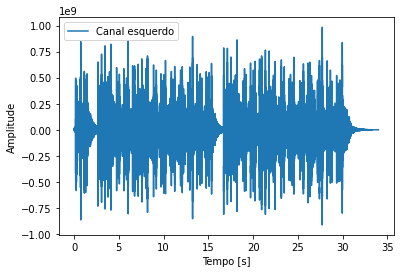
\includegraphics[width = \columnwidth]{elise_frequency.png}
            \end{figure}
            
        \column{0.5 \textwidth}
        \begin{figure}
            \centering
            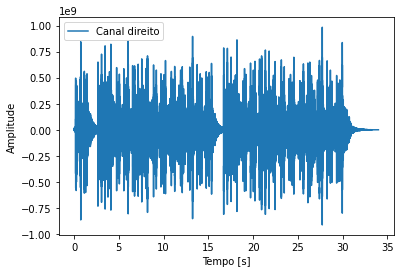
\includegraphics[width = \columnwidth]{elise_frequency.2png.png}
        \end{figure}
    \end{columns}
\end{frame}

\begin{frame}{Espectro de frequências}

Função rfft da biblioteca scipy. N = 16 320 000. Eixo x: frequência digital.

\begin{figure}
    \centering
    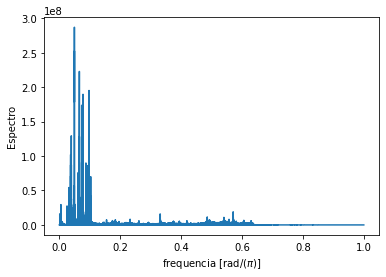
\includegraphics[scale = 0.7]{freq_espectro.png}
\end{figure}
    
\end{frame}

\begin{frame}{Espectro de frequências}
Função welch, fs = 2. 
\begin{figure}
    \centering
    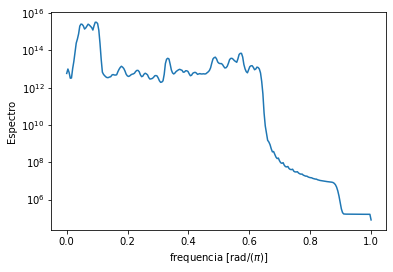
\includegraphics[scale = 0.7]{welsh_espectro.png}
\end{figure}
\end{frame}

\begin{frame}{Filtro FIR}
Especificações do filtro.
\begin{itemize}
    \item $\omega_c = \frac{\pi}{2}$
    \item $\Delta \omega \leq 0.05 \pi$  
    \item Erro na faixa de passagem e rejeição $\leq 0.001 = -60$ dB
\end{itemize}
\end{frame}

\begin{frame}{Janela de Kaiser}
     \begin{align*}
         &A = -20\log (0.001) = 60 \\ \\
         &\beta = 0.1102\cdot(A - 8.7) = 5.6326 \\ \\
         &M = \frac{A - 8}{2, 285\Delta \omega} = 146
     \end{align*}
\end{frame}

\begin{frame}{Filtro FIR}
    Pyfda.
    \begin{figure}
        \centering
        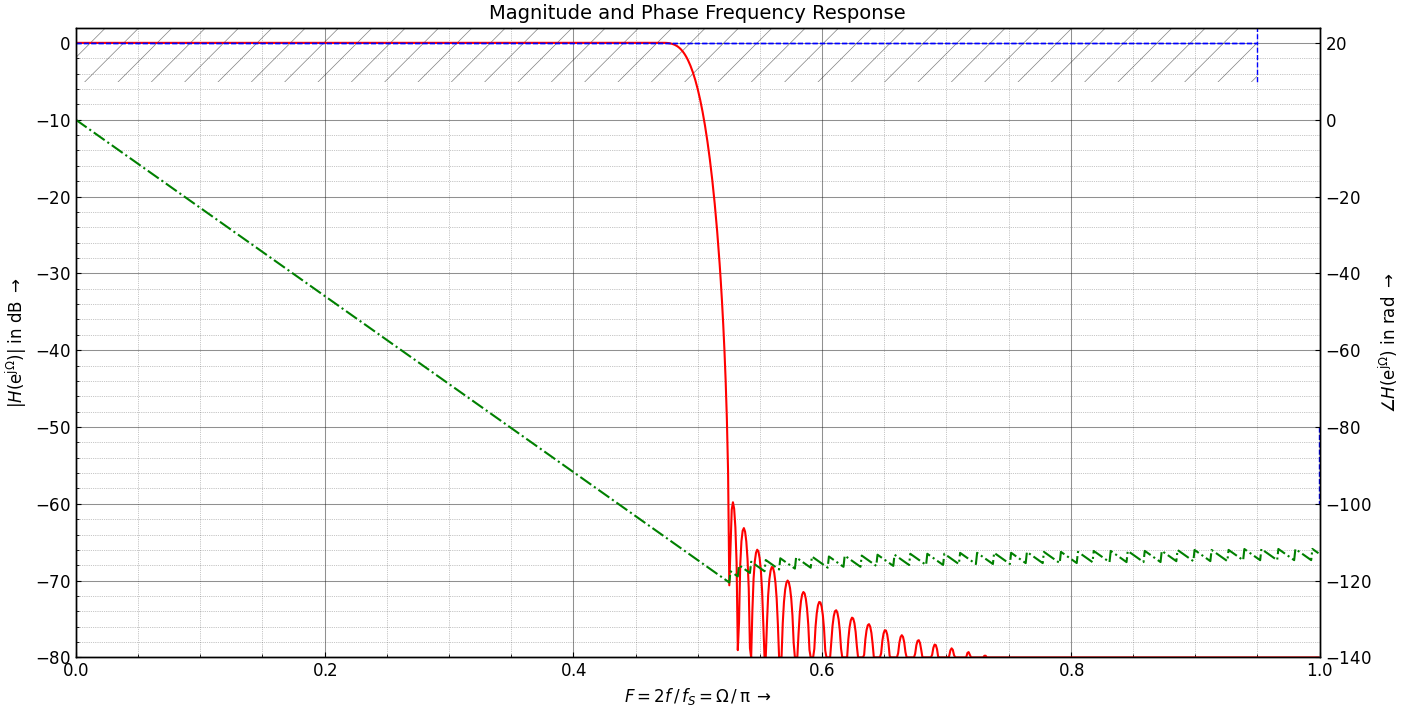
\includegraphics[scale=0.33]{filtro_fase.png}
    \end{figure}
\end{frame}

\begin{frame}{Sistema SLIT}
    Overlap and add. \\
    \begin{itemize}
        \item x[n] é dividido em $r$ blocos de comprimento $L$.
        \item $x_r[n]$ é convoluído com $h[n]$ no domínio da frequência (FFT).
        \item $y_r$ é recuperado através da IFFT,
        \item  As partes de $y_r$ que se sobrepõem são somadas, formando $y = x * h$
    \end{itemize}
      
\end{frame}

\begin{frame}{Overlap and add}
     \begin{figure}
         \centering
         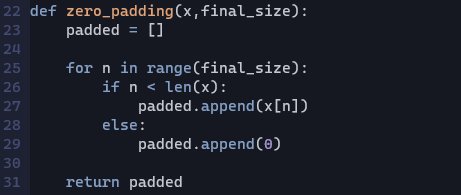
\includegraphics[scale = 1.0]{padding.png}
     \end{figure}
\end{frame}

\begin{frame}{Overlap and add}
     \begin{figure}
         \centering
         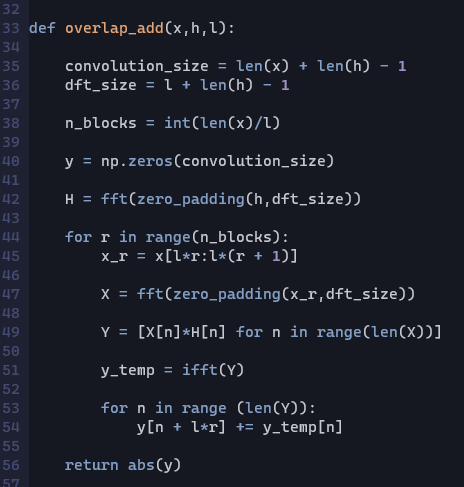
\includegraphics[scale = 0.75]{overlap.png}
     \end{figure}
\end{frame}

\begin{frame}{Complexidade - Overlap and add}
    Seja x[n] dividido em $r$ blocos de tamanho L. Para cada bloco 
    \begin{itemize}
        \item DFT e IDFT $\rightarrow  2 \cdot \frac{N}{2}\log_2{(N)}$ 
        \item Produto X[k]H[k] $\rightarrow N \log_2{(N)} + N = N \log_2{(2N)}$ 
    \end{itemize}
    Dado que cada multiplicação complexa utiliza 4 produtos reais:
    \begin{equation*}
        c = 4\frac{N \log_2{(2)}}{L}
    \end{equation*}
    Por ponto, onde N = L + K - 1. 
\end{frame}


\begin{frame}{Complexidade - Overlap and add}
    Dado que a FFT requer que o tamanho da DFT seja uma potência de 2:
    \begin{align*}
        c &= 4\frac{N \log_2{(2)}}{L} \\ \\
        c &= 4\frac{2^i(i + 1)}{2^i - K + 1} \\ \\
    \end{align*}
    Assim, dado um filtro FIR de K coeficientes, o valor ótimo de L é aquele que minimiza c. 
\end{frame}

\begin{frame}{Complexidade Overlap and add}
Dado que o filtro fir projetado tem 147 estágios.
\begin{figure}
    \centering
    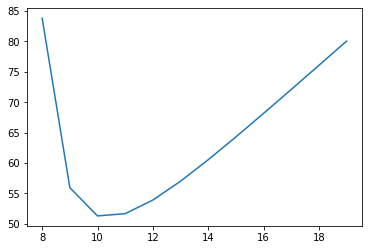
\includegraphics[scale = 0.6]{complexidade.png}
\end{figure}
Portanto, $L = 2^{10} - 147 + 1 = 878$ é a escolha mais eficiente.  
\end{frame}

\begin{frame}{Filtragem}
    \begin{figure}
        \centering
        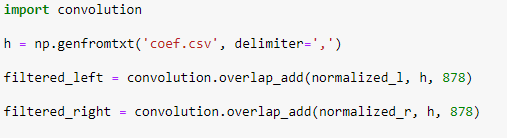
\includegraphics[scale = 1]{finalmente.png}
    \end{figure}
\end{frame}

\begin{frame}{Filtragem - welch}
    \begin{figure}
        \centering
        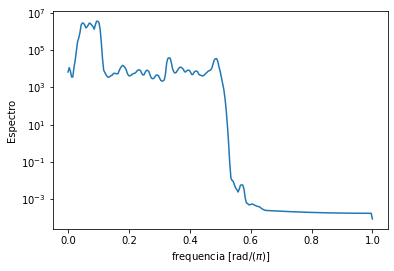
\includegraphics[scale = .8]{filtered_welsh.png}
    \end{figure}
\end{frame}

\begin{frame}{Filtragem - FFT}
    \begin{figure}
        \centering
        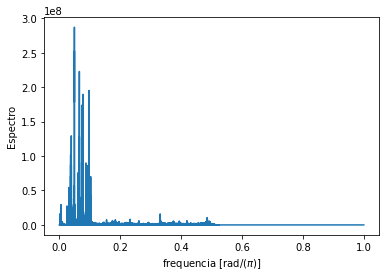
\includegraphics[scale = .8]{filtered_fourier.png}
    \end{figure}
\end{frame}


\begin{frame}{Domínio do tempo - sinais filtrados}
    \begin{columns}
        \column{0.5 \textwidth}
            \begin{figure}
                \centering
                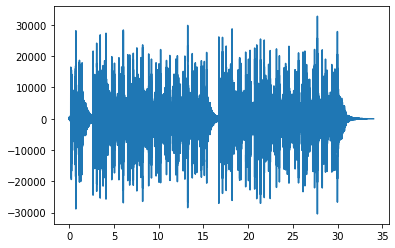
\includegraphics[width = \columnwidth]{tempo_filtro1.png}
            \end{figure}
            
        \column{0.5 \textwidth}
        \begin{figure}
            \centering
            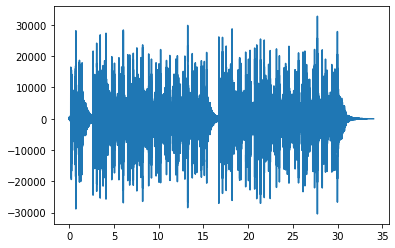
\includegraphics[width = \columnwidth]{tempo_filtro2.png}
        \end{figure}
    \end{columns}
\end{frame}

\begin{frame}{Interpolação do sinal}
   \begin{itemize}
       \item Upsampling - 2
       \item FPB - Corte $\omega_c = \frac{\pi}{2}$ e Ganho = 2
   \end{itemize}
\end{frame}

\begin{frame}{Upsampling}
    \begin{figure}
        \centering
        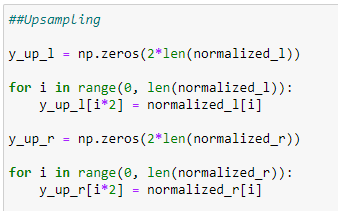
\includegraphics[scale = 1.0]{upsampling.png}
    \end{figure}
\end{frame}

\begin{frame}{Filtragem}
    \begin{figure}
        \centering
        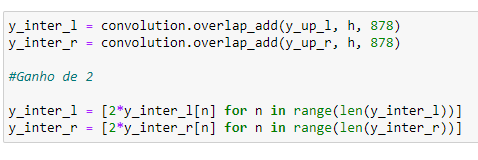
\includegraphics[scale = 1.0]{filtrage.png}
    \end{figure}
\end{frame}
\begin{frame}{Interpolação do sinal - Domínio da frequência}
   \begin{figure}
        \centering
        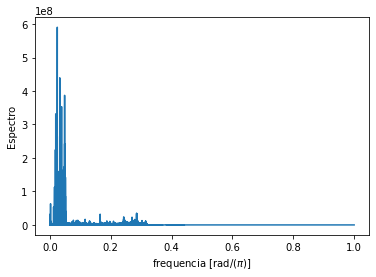
\includegraphics[scale = .8]{interpol1.png}
    \end{figure}
\end{frame}

\begin{frame}{Interpolação do sinal - Domínio do tempo}
   \begin{columns}
        \column{0.5 \textwidth}
            \begin{figure}
                \centering
                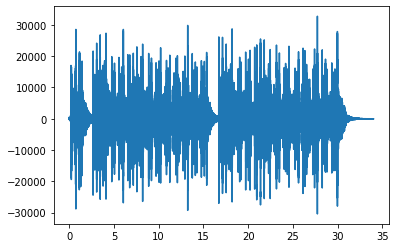
\includegraphics[width = \columnwidth]{interpol_time.png}
            \end{figure}
            
        \column{0.5 \textwidth}
        \begin{figure}
            \centering
            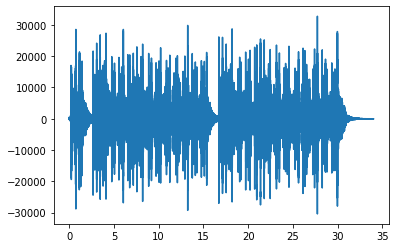
\includegraphics[width = \columnwidth]{interpol_tim2.png}
        \end{figure}
    \end{columns}
\end{frame}

\end{document}
